%-----------------------------------------------------------------------------%
\chapter{\babTiga}
%-----------------------------------------------------------------------------%
Bagian ini akan menjelaskan mengenai metodologi penelitian yang digunakan dalam penelitian ini. Metodologi tersebut meliputi pendekatan penelitian, populasi dan sampel penelitian, tahapan penelitian, model penelitian, instrumen penelitian, metode pengumpulan data, hipotesis awal dan teknik analisis data.
%-----------------------------------------------------------------------------%
\section{Pendekatan Penelitian}
%-----------------------------------------------------------------------------%
Penelitian dilakukan dengan menggunakan pendekatan secara kuantitatif dan kualitatif. Pendekatan kuantitatif adalah suatu teknik pengumpulan data melalui media-media yang telah ditentukan dan menghasilkan data statistik \citep{buku.creswell}. Creswell menjelaskan bahwa terdapat dua strategi yang dapat dilakukan pada pendekatan kuantitatif, yaitu eksperimen dan survei. Dalam penelitian ini penulis melakukan eksperimen dengan pelaksanaan \ust. Selanjutnya pendekatan kualitatif adalah suatu teknik pengumpulan data dan analisis terhadap data-data yang sifatnya tidak numerik. Pada penelitian ini diperoleh data yang bersifat kuantitatif dimana diperoleh dari tanggapan responden terhadap \f{website} melalui kuesioner dengan skala likert serta data kualitatif yang diperoleh dari preferensi, rekomendasi dan saran responden terhadap \f{website}.
%-----------------------------------------------------------------------------%
\section{Populasi dan Sampel}
%-----------------------------------------------------------------------------%
Populasi yang digunakan dalam penelitian ini adalah mahasiswa dengan jurusan Administrasi di lingkungan Universitas Indonesia, konsultan pajak dan pekerja di bidang pajak. Populasi ini dipilih berdasarkan pada pemahaman dan kebutuhan pengguna terhadap \f{website} direktorat jenderal pajak. Adapun sampel pada penelitian ini adalah 35 orang terpilih dari populasi dengan komposisi 10 orang mahasiswa serta 25 orang konsultan dan pekerja di bidang pajak. Pemilihan sampel dalam penelitian ini menggunakan metode \textit{purposive sampling}, dimana penulis mencari responden yang sesuai dengan kriteria pada populasi. Adapun kriteria dalam penelitian ini adalah mahasiswa dan pekerja di bidang pajak yang sudah pernah membuka \f{website} direktorat jenderal pajak Indonesia.
%-----------------------------------------------------------------------------%
\section{Tahapan Penelitian}
%-----------------------------------------------------------------------------%
Tahapan yang dilakukan pada penelitian ini adalah perumusan masalah, studi literatur, penyusunan rancangan penelitian, pengumpulan data (eksperimen), analisis data, perancangan \f{prototype}, evaluasi \f{prototype}, dan penarikan kesimpulan.
%-----------------------------------------------------------------------------%
\subsection{Perumusan Masalah}
Pada tahap ini dilakukan perumusan masalah yang akan diangkat dalam penelitian. Permasalahan yang diangkat adalah kemudahan, kenyamanan dan fungsionalitas penggunaan sistem \f{e-government} berbasis \f{website} melalui tampilan antarmuka dan \f{user experience}. Kenyamanan, kemudahan dan fungsionalitas ini ditujukan untuk meningkatkan produktifitas pengguna dalam menggunakan sistem serta pelayanan dari sistem yang semakin baik.
%-----------------------------------------------------------------------------%
\subsection{Studi Literatur}
Pada tahap ini dilakukukan studi literatur dengan cara pencarian definisi dan teori penunjang. Hasil pencarian digunakan untuk pembuatan model penelitian yang dilakukan. Proses studi literatur yang dilakukan meliputi teori \f{e-government}, pengujian \f{e-government}, \ust, \f{website} direktorat jenderal pajak serta teori lainnya yang berkaitan dengan permasalahan pada penelitian.
%-----------------------------------------------------------------------------%
\subsection{Penyusunan Rancangan Penelitian}
Pada tahap ini dilakukan penyusunan rancangan penelitian. Rancangan penelitian terdiri dari beberapa komponen dengan menjalankan \ust. Komponen-komponen tersebut adalah sebagai berikut:
%-----------------------------------------------------------------------------%
\subsubsection{Mengembangkan \f{Test Plan}}
\f{Test plan} dalam \ust \space merupakan tahapan yang penting dimana menurut \citet{buku.rubin} \f{test plan} berfungsi sebagai peta pengujian, kendaraan komunikasi yang utama,  menyiratkan kebutuhan dasar, dan juga menyediakan titik fokus pengujian menjadi sebuah pencapaian. \citeauthor{buku.rubin} menjabarkan \f{test plan} menjadi beberapa bagian seperti berikut:
\begin{enumerate}[label=\alph*.]
	\item Menentukan maksud, capaian dan tujuan dari \f{test}\\
	Pada tahap ini ditinjau kembali maksud dan tujuan dari \ust \space serta meninjau ulang capaian yang ingin diraih dari hasil pengujian. Bagian ini akan dijelaskan pada subbab 3.3.1 dan subbab 3.3.6.
	\item Menentukan target pengguna\\
	Tahap ini menjelaskan mengenai target pengguna yang akan menjadi responden dalam proses \ust. Pengguna dalam penelitian ini merupakan refleksi dari pengguna sistem. Pengguna yang dipilih menjadi responden \ust \space ini telah dijelaskan pada subbab 3.2.
	\item Menentukan dan menetapkan metode \f{test design}\\
	Pada tahap ini dilakukan penetapan dan penentuan \f{test} yang akan dilakukan. Proses penentuan dan penetapan meliputi prosedur \f{testing} dan prosedur pengumpulan data. Berikut merupakan prosedur yang dilakukan dalam penelitian ini:
	\begin{itemize}
		\item Proses pengumpulan data dilakukan pada tanggal 18 Mei 2015 sampai dengan 1 Juni 2015.
		\item \f{Usability testing} dilakukan dengan menggunakan komputer pribadi milik penulis ataupun pengguna yang sudah disiapkan sebelumnya. 
		\item Penulis selaku penguji membebaskan kepada responden untuk melakukan eksplorasi terhadap sistem \f{website} selama pengerjaan tugas yang telah diberikan.
		\item Penulis selaku penguji hanya bertindak mengamati dan menjadi moderator selama pengujian.
	\end{itemize} 
	\item Merancang dan Menentukan daftar tugas dan kuesioner pengujian\\
	Pada bagian ini penulis melakukan perancangan terkait tugas dan kuesioner yang akan kepada responden dalam \ust. Deskripsi lebih lanjut mengenai tahap ini akan dijelaskan pada subbab 3.3.3.2.
	\item Menyiapkan lingkungan penelitian dan perlengkapan pengujian\\
	Pada tahap ini ditentukan persiapan untuk melaksanakan penelitian (pengumpulan data). Lingkungan penelitian yang disiapkan penulis adalah lokasi yang kondusif untuk melakukan moderasi, seperti tempat yang memiliki ruang gerak cukup luas. Perlengkapan yang disiapkan penulis dalam melaksanakan \ust \space adalah sebagai berikut:
	\begin{itemize}
		\item 1 buah PC yang akan digunakan responden dalam \ust,
		\item Skenario pengujian,
		\item Kuesioner dan
		\item \f{Stopwatch}
	\end{itemize}
\end{enumerate}
%-----------------------------------------------------------------------------%
\subsubsection{Perancangan tugas dan kuesioner}
Dalam perancangan tugas penulis memakai acuan berdasar fitur yang dimiliki oleh \f{website} direktorat jenderal pajak baik Indonesia maupun India. Fitur yang memiliki kesamaan kemudian dikelompokkan menjadi poin tugas yang akan dilakukan oleh responden. Tugas-tugas disusun berdasar dengan materi komponen pengujian yang sudah dijelaskan pada subbab 2.2.2.
Berikut merupakan daftar tugas yang diberikan pada responden:
\begin{enumerate}
	\item Melakukan pengamatan halaman utama sistem \f{website},
	\item Pengamatan Desain halaman artikel dan fitur arsip artikel,
	\item Melakukan pengunduhan berkas dari arsip unduhan,
	\item Eksplorasi halaman bantuan dan dokumentasi,
	\item Eksplorasi halaman terkait pengumuman,
	\item Eksplorasi halaman keterbukaan informasi terkait informasi lelang,
	\item Menggunakan sistem pencarian \f{website} berdasar kata kunci,
	\item Pencarian kontak informasi,
	\item \f{Login} aplikasi \f{e-filling} dan melakukan kegiatan pengamatan beserta eksplorasi fitur yang ada, seperti pengelolaan item form yang ada dan \f{logout} sistem, serta
	\item Uji coba pranala yang berkaitan dengan sistem.
\end{enumerate}
Penyusunan tugas yang diberikan terhadap responden telah diatur sedemikian rupa agar mereprentasikan tujuan dalam penelitian ini. Tugas tersebut diproyeksikan kedalam skenario pengujian.
\newline\\
Untuk melaksanakan pengujian terhadap \f{website} \f{e=government}, dirancang sebuah kuesioner yang dapat mengumpulkan data penilaian \f{website}. Kuesioner ini disusun berdasarkan komponen-komponen yang dijabarkan pada subbab 2.2.2 dan 2.1.3. Adapun rancangan kuesioner \ust \space terdiri dari beberapa bagian sebagai berikut:
\begin{enumerate}
	\item Biodata Responden\\
	Pada bagian ini kuesioner berisikan mengenai biodata dan informasi terkait responden yang dibutuhkan untuk tahap analisis demografi.
	\item Komponen \f{Usability}\\
	Bagian komponen \f{usability} berfungsi sebagai alat ukur untuk mendapatkan nilai \f{usability heuristic}. Berikut merupakan tabel pertanyaan dari kuesioner komponen \f{usability heuristic} yang diberikan kepada responden:
	\begin{table}[h]
		\centering
		\caption{Tabel Kuesioner Komponen \f{Usability Heuristic} }
		\begin{tabular}{|p{11.2cm}|}
			\hline
			\multicolumn{1}{|c|}{{\bf Pertanyaan}}\\  
			\hline
			{\bf Visibility of system status}                                                                           \\
			Feedback yang diberikan sistem membuat saya mengetahui apa yang sedang saya lakukan.                        \\ \hline
			{\bf Match between system and real world}                                                                   \\
			Istilah yang digunakan sudah jelas deskriptif dan familiar bagi saya.                                       \\
			Informasi yang diberikan mudah dimengerti.                                                                  \\ \hline
			{\bf User control}                                                                                          \\
			Saya dapat melakukan pembatalan terhadap suatu task.                                                        \\ \hline
			{\bf Consistency and standards}                                                                             \\
			Istilah jenis font dan design yang digunakan konsisten.                                                     \\ \hline
			{\bf Error prevention}                                                                                      \\
			Saya mengerti keterangan yang diberikan pada sistem.                                                        \\
			Keterangan pada sistem membuat saya tidak melakukan kesalahan.                                              \\ \hline
			{\bf Recognition rather than recall}                                                                        \\
			Letak menu dan icon yang digunakan membantu saya untuk mengetahui tujuan dan fungsinya.                     \\
			Saya dapat mengingat dengan mudah bagaimana cara menggunakan sistem.                                        \\ \hline
			{\bf Flexibility and efficiency of use}                                                                     \\
			Saya mengerti tujuan dari sistem ini secara keseluruhan.                                                    \\
			Saya mengerti tujuan dari menu yang digunakan.                                                              \\
			Saya dapat menggunakan sistem dengan mudah.                                                                 \\ \hline
			{\bf Aesthetic and Minimalist Design}                                                                       \\
			Setelah menggunakan sistem saya menilai sistem ini menarik (dari segi tampilan dan tata letak).             \\
			Saya tidak keberatan untuk berlama-lama menggunakan sistem ini.                                             \\ \hline
			{\bf Help user recognize diagnose and recover from errors}                                                  \\
			Ketika saya melakukan kesalahan sistem memberikan petunjuk sehingga saya dapat memperbaikinya dengan mudah. \\ \hline
			{\bf Help and documentation}                                                                                \\
			Informasi tambahan (fitur help/FAQ) membuat saya mengerti ketika mengalami kesulitan.                       \\ \hline
		\end{tabular}
	\end{table}
	\item Komponen Kepuasan Pengguna\\
	Komponen ini menjelaskan mengenai kepuasan pengguna terhadap \f{website} yang dievaluasi. Berikut merupakan tabel pertanyaan kepuasan pengguna yang terdapat dalam kuesioner:
	\begin{table}[h]
		\centering
		\caption{Tabel Kuesioner Komponen Kepuasan Pengguna}
		\begin{tabular}{|p{11.2cm}|}
			\hline
			\multicolumn{1}{|c|}{{\bf Pertanyaan}}						\\ \hline
			Saya merasa mudah dan nyaman untuk menggunakan sistem ini.	\\ \hline
			Saya membutuhkan sistem ini untuk membantu pekerjaan saya.	\\ \hline
			Saya akan merekomendasikan sistem ini kepada orang lain.	\\ \hline
		\end{tabular}
	\end{table}
	\item Komponen \f{g-Quality}\\
	Komponen ini merupakan komponen untuk mengevaluasi nilai \f{website} \f{e-government} berdasarkan kategori yang sudah dijelaskan pada subbab 2.1.3. Berikut merupakan tabel pertanyaan komponen \f{g-quality} yang terdapat pada kuesioner:
	\begin{table}[h]
		\centering
		\caption{Kuesioner Komponen Kepuasan Pengguna}
		\begin{tabular}{|p{11.2cm}|}
			\hline
			\multicolumn{1}{|c|}{{\bf Pertanyaan}}										\\ \hline
			{\bf Accessibility}															\\
			Sistem dapat digunakan dan dioperasikan oleh semua kalangan.               	\\ \hline
			{\bf Interoperability}                                                      \\
			Dapat melakukan pertukaran data dan informasi dengan sistem E-Gov lainnya.  \\ \hline
			{\bf Security and Privacy}                                                  \\
			Sistem dapat mencegah terjadinya kebocoran data yang dimiliki pengguna.     \\ \hline
			{\bf Information Truth and Precision}                                       \\
			Saya merasa sistem menyampaikan informasi yang benar, akurat dan terkini.   \\ \hline
			{\bf Service Agility}                                                       \\
			Saya merasa penggunaan sistem cepat dan mudah diakses.                      \\ \hline
			{\bf Transparency}                                                          \\
			Saya merasa informasi yang disampaikan sistem sudah transparan.				\\ \hline
		\end{tabular}
	\end{table}
\end{enumerate}
%-----------------------------------------------------------------------------%
\subsubsection{Menentukan tipe data}
Tipe data yang digunakan dalam penelitian ini adalah sebagai berikut:
\begin{enumerate}
	\item Kuantitatif\\
	Tipe data kuantitatif terdiri dari waktu yang dibutuhkan responden dalam pengerjaan tugas dan juga penilaian yang diberikan responden terhadap komponen pengujian dalam kuesioner.
	\item Kualitatif\\
	Tipe data kualitatif pada penelitian ini terdiri dari penilaian tertulis, rekomendasi dan saran dari responden terhadap \f{website} dan \f{prototype}.
\end{enumerate}
%-----------------------------------------------------------------------------%
\subsubsection{Persiapan pelaksanaan \ust}
Sebelum melaksanakan \ust, penulis selaku penguji melakukan beberapa aktifitas seperti \f{checklist} dalam persiapan pengujian seperti yang disampaikan \citet{buku.rubin}. Berikut merupakan daftar \f{checklist} yang dilakukan penulis dalam persiapan pelaksanaan pengujian:
\begin{enumerate}
	\item \f{Checklist 1: Test Preparation}\\
	Sebelum masuk ke masa pengujian, penulis melakukan \f{selftest} dan \f{pilot test} terlebih dahulu dengan tujuan memberikan gambaran pada saat pengujian yang akan dilaksanakan nanti. Berikut merupakan tahapan yang dilakukan pada \f{test preparation} ini:
	\begin{itemize}
		\item Melakukan \f{self test} untuk menyesuaikan skenario pengujian dengan sistem yang akan diujikan.
		\item Melaksanakan \f{pilot test} yang dilakukan oleh satu orang sukarelawan untuk menguji skenario dan pelaksanaan \ust \space sebagai simulasi. 
		\item Melakukan uji keterbacaan kuesioner dan skenario bersama 5 orang sukarelawan secara acak dengan maksud mendapat \f{feedback} untuk dilakukan perbaikan nantinya.
		\item Revisi kuesioner dan skenario berdasarkan pengujian pada tahap sebelumnya.
	\end{itemize}
	\item \f{Checklist 2: Pre-test}\\
	Penulis melakukan persiapan sebelum melaksanakan pengujian terhadap responden dengan mempersiapkan perlengkapan seperti PC siap pakai, jaringan yang sudah terkoneksi dan membagikan skenario \f{testing} yang telah disiapkan.
	\item \f{Checklist 3: Test Monitor Activities}\\
	Penulis melakukan monitoring dan moderasi pada saat pelaksanaan \ust. Aktifitas monitoring ini ditujukan untuk memastikan data sudah terisi dengan benar serta melakukan rekap data terkait kesalahan, waktu dan catatan selama \ust \space berlangsung.
\end{enumerate}
%-----------------------------------------------------------------------------%
\subsection{Pelaksanaan Penelitian}
Pada tahap ini penulis melakukan \ust \space terhadap \f{website} \f{e-government} dengan mengikuti aturan yang dijelaskan oleh \citet{buku.rubin} dan \citet{buku.dumas} sebagai berikut:
\begin{enumerate}
	\item Perkenalan\\
	Pada bagian ini penulis melakukan perkenalan terhadap responden dan menjelaskan mengenai latar belakang penelitian, skenario \f{testing} dan pengisian kuesioner.
	\item \f{Pre-test briefing}\\
	Sebelum memasuji sesi pengujian, penulis melakukan \f{briefing} terhadap responden yang menjelaskan mengenai kegiatan yang akan dilakukan dan mempersilahkan responden untuk melakukan eksplorasi terhadap \f{website} yang diujikan.
	\item Sesi \f{test}\\
	Pada saat sesi ini responden menjalankan tugas sesuai dengan skenario yang telah disiapkan sebelumnya. Penulis bertugas menjadi moderator dan fasilitator pada saat \f{test} berjalan.
	\item \f{Post-test debriefing}\\
	Setelah sesi pengujian selesai dilakukan oleh responden, penulis menjelaskan kembali terkait cara pengisian kuesioner dan memandu responden dalam melakukan pengisian kuesioner yang telah diberikan.
\end{enumerate}
%-----------------------------------------------------------------------------%
\subsection{Analisis Data dan \f{Requirement Gathering}}
Pada tahap ini dilakukan analisis data dari hasil \ust \space dengan responden  dengan metode yang akan dijelaskan pada subbab 3.5 dan mengumpulkan \f{requirement} dari hasil analisis rekomendasi responden untuk mengembangkan \f{clickable-prototype}. 
%-----------------------------------------------------------------------------%
\subsection{Perancangan \f{Prototype}}
Pada tahap ini penulis melakukan perancangan \f{prototype} yang dibuat berdasarkan hasil \ust \space dengan responden. Penulis mengembangkan prototype dengan aplikasi berbasis web \textbf{proto.io} yang sudah dijelaskan pada subbab 2.8. 
%-----------------------------------------------------------------------------%
\subsection{Evaluasi \f{Prototype}}
Setelah melakukan pengembangan \f{clickable-prototype}, penulis akan mengevaluasi \f{prototype} kepada 1/3 responden terpilih dengan menggunakan A/B Testing. Dimana menurut \citet{article.rohrer} A/B testing adalah metode ilmiah dalam pengujian desain berbeda pada sebuah \f{website} kepada sekelompok responden acak untuk berinteraksi dengan desain berbeda serta mengukur pengaruh tugas terhadap perilaku pengguna.
%-----------------------------------------------------------------------------%
\section{Metode Pengumpulan Data}
%-----------------------------------------------------------------------------%
Pada bagian ini akan dijelaskan mengenai metode pengumpulan data beserta jenis dan sumber data yang digunakan pada penelitian.  
%-----------------------------------------------------------------------------%
\subsection{Jenis dan Sumber Data}
Penelitian ini menggunakan sumber data primer yang diperoleh langsung dari orang pertama, yakni dari responden secara langsung. Penelitian ini menggunakan dua jenis data, yaitu data subjektif dan data objektif.
\begin{enumerate}
	\item Data Subjektif\\
	Data subjektif dalam penelitian ini diperoleh dari kuesioner yang menggunakan skala likert serta rekomendasi dan saran dari responden. Skala likert digunakan sebagai penilaian subjektif responden terhadap \f{website} \f{e-government} yang diujikan dan rekomendasi sebagai bagian dari masukkan responden untuk peningkatan fitur atau aspek tertentu dari \f{website} yang diujikan. 
	\item Data Objektif\\
	Data objektif dalam penelitian ini diperoleh dari hasil pengukuran data kuantitatif yang diakukan oleh penulis sebagai moderetor dan fasilitator dalam pelaksanaan \ust. Data objektif meliputi waktu pengerjaan tugas selama pengujian dan jumlah kesalahan tugas yang dilakukan oleh responden.
\end{enumerate}
%-----------------------------------------------------------------------------%
\subsection{Teknik Pengumpulan Data}
Penulis melakukan beberapa cara untuk melakukan pengumpulan data seperti berikut:
\begin{enumerate}
	\item Observasi\\
	Metode ini digunakan pada saat melakukan penelitian dengan mengumpulkan data secara langsung melalui pengamatan terhadap responden pada saat \ust \space berlangsung. Observasi yang dilakukan adalah melihat, mengukur waktu, menghitung serta mencatat kejadian yang ada pada saat \ust. Pengukuran waktu dilakukan dengan menghitung waktu kinerja responden dalam pengerjaan tugas secara keseluruhan, sedangkan penghitungan dilakukan dengan mencatat jumlah kesalahan dan masalah yang dialami oleh responden.
	\item Kuesioner\\
	Kuesioner dideskripsikan oleh \citet{buku.riduwan} sebagai daftar pertanyaan yang diberikan kepada orang lain yang bersedia memberikan respons (responden) sesuai dengan permintaan pengguna. \citeauthor{buku.riduwan} menjelaskan tujuan dari kuesioner adalah untuk mencari informasi yang lengkap mengenai suatu masalah dan reponden tidak merasa khawatir bila memberikan jawaban yang diberikan tidak sesuai dengan kenyataan dalam pengisian daftar pertanyaan.
	Adapun jenis pertanyaan yang disajikan pada kuesioner yaitu \citep{buku.riduwan}:
	\begin{enumerate}
		\item Pertanyaan terbuka\\
		Kuesioner dengan jenis pertanyaan terbuka (tidak memiliki struktur) adalah kuesioner yang disajikan dalam bentuk sederhana sehingga responden dapat memberikan isian sesuai dengan kehendak dan keadaannya. Dalam penelitian ini terdapat bagian dari kuesioner yang memiliki pertanyaan terbuka seperti pada bagian rekomendasi dan preferensi responden.
		\item Pertanyaan tertutup\\
		Pertanyaan tertutup dijelaskan sebagai kuesioner yang disajikan dalam bentuk sedemikian rupa sehingga responden diminta untuk memilih satu jawaban yang sesuai dengan karakteristik dirinya dengan cara menandai pilihan (dapat berupa skala atau pilihan ganda) pada pertanyaan. Pada penelitian ini digunakan skala likert sebagai pilihan yang terdapat pada kuesioner. Skala likert adalah skala yang digunakan untuk mengukur sikap, pendapat dan persepsi seseorang atau sekelompok tentang kejadian atau gejala sosial \citep{buku.riduwan}. Skala likert yang digunakan penulis adalah sebagai berikut:
		\begin{table}[h]
			\centering
			\caption{Skala Likert pada Kuesioner}
			\label{tab:tab2}
			\begin{tabular}{|c|l|}
				\hline
				{\bf Skala} & \multicolumn{1}{c|}{{\bf Keterangan}} \\ \hline
				1           & Sangat tidak setuju                   \\ \hline
				{\it 2}     & Tidak setuju                          \\ \hline
				3           & Agak tidak setuju                     \\ \hline
				{\it 4}     & Netral                                \\ \hline
				5           & Agak setuju                           \\ \hline
				6           & Setuju                                \\ \hline
				7           & Sangat setuju                         \\ \hline                      
			\end{tabular}
		\end{table}
	\end{enumerate}
\end{enumerate}
%-----------------------------------------------------------------------------%
\section{Metode Analisis Data}
Metode analisis data yang digunakan pada penelitian ini adalah metode statistik \f{paired samples t-test} yang melakukan uji rata-rata pada dua buah kelompok data yang saling berhubungan. Data yang diolah dalam metode ini adalah data yang bersifat parametrik dengan bentuk interval dan terdistribusi secara normal. Diperlukan uji normalitas untuk melihat apakah data terdistribusi secara normal. Dikarenakan data dalam penelitian ini bersifat ordinal dengan skala kategori lebih dari 4, maka penulis tidak perlu melakukan konversi nilai ordinal menjadi interval karena menurut \citet{paper.jason} data ordinal dengan skala kategori lebih dari 5 dapat langsung dihitung dan dianalisa dengan metode parametrik.
%-----------------------------------------------------------------------------%
\subsection{Uji Normalitas}
Uji normalitas bertujuan untuk menguji apakah data terdistribusi normal. \citet{ppt.schwab} mengatakan bahwa terdapat dua cara untuk mengevaluasi normalitas. Pertama adalah dengan metode statistikal, lalu kedua menggunakan pengamatan grafis. Metode grafis menggunakan histogram dan plot normalitas dalam pengamatannya. Gambar \ref{fig:histogramnormal} menunjukan histogram yang terdistribusi normal. Sedangkan metode statistikal melakukan diagnosa hipotesis tes untuk normalitas dan variabelnya mendekati normal jika \f{skewnes} dan \f{kurtosis} memiliki nilai antara -2.0 dan 2.0, gambar \ref{fig:grafiknormal} menunjukan grafik dataset yang terdistribusi normal. Menurut \citet{buku.sugiyono}, salah satu uji normalitas data adalah dengan metode chi kuadrat ($x^2$) dimana pengujian hipotesis dilakukan dengan cara membandingkan kurva normal yang terbentuk dari data yang telah terkumpul (B) dengan kurva normal standar (A). Bila B tidak berbeda secara signifikan dengan A, maka B merupakan data yang berdistribusi normal. Cara lain untuk melakukan uji normalitas adalah dengan metode deskriptif, dimana metode ini menghitung \f{skewness} dan nilai \f{kurtosis}, setelah itu dilakukan transformasi kedua nilai tersebut dengan \f{z-score}. 
\newline\\
Suatu besaran statistik yang menunjukan kemiringan data disebut \f{skewness}, data \f{skewnes} memiliki kecenderungan berada di tengah atau miring di satu sisi saja. Sedangkan \f{kurtosis} merupakan keruncingan data \citep{article.setiawan}. Rasio \f{skewnes} dapat diperoleh dari rumus:
\begin{equation}
\centering
 Z_{skewnes} = \cfrac{s-0}{SE_{skewness}} 
\end{equation}
Dengan nilai \f{skewness} adalah \f{s} dan SE nilai \f{standard error}. Data terdistribusi normal jika berada pada rentang -1.0 sampai 1.0. Sedangkan nilai rasio kurtosis dapat diperoleh dengan persamaan berikut:
\begin{equation}
\centering
Z_{kurtosis} = \cfrac{s-0}{SE_{skewness}} 
\end{equation}

\begin{figure}[ht]
	\centering
	\begin{minipage}[b]{0.45\linewidth}
		\centering
		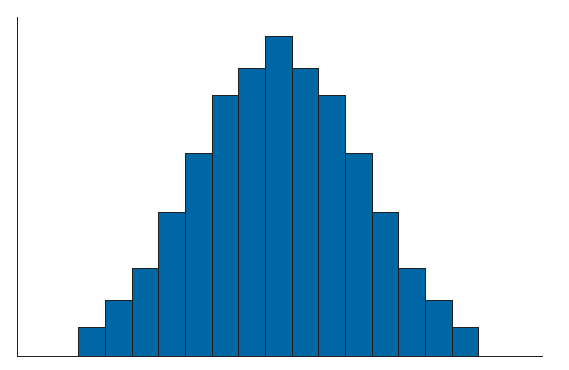
\includegraphics[width=\textwidth]{pics/histogram-normal.png}
		\caption{Histogram \f{Normal Distribution Dataset}}
		\label{fig:histogramnormal}
	\end{minipage}
	\hspace{0.5cm}
	\begin{minipage}[b]{0.45\linewidth}
		\centering
		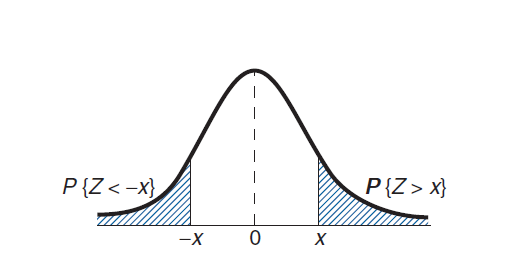
\includegraphics[width=\textwidth]{pics/normal-distribution.png}
		\caption{Grafik \f{Normal Distribution Dataset}}
		\label{fig:grafiknormal}
	\end{minipage}
\end{figure}
\begin{center}
	{\small Sumber gambar: \citep{buku.ross}}
\end{center}
Bila data tidak terdistribusi secara normal, maka dapat dilakukan uji normalisasi dengan mentransformasi data. Transformasi data dapat dilakukan dengan aplikasi SPSS pada menu "Compute Variable". \citet{buku.field} menjelaskan bahwa penghitungan uji normalitas pada SPSS dapat dilakukan dengan cara seperti berikut:
\begin{enumerate}
	\item \f{Log Transformation}\\
	Bila data bersifat \f{positive skew} maka digunakan metode ini untuk memperbaiki data yang memiliki \f{unequal variances}. Bila data memiliki nilai 0 atau bernilai negatif, maka dilakukan $log(X_{1}+1)$ untuk membuat data tetap positif.
	\item \f{Square Root Transformation}\\
	Metode ini digunakan untuk mengurai \f{positive skew} dengan mengambil akar kuadrat dari masing-masing data. Metode ini memiliki kekurangan ketika mengurai data yang memiliki nilai negatif, hal ini disebabkan nilai negatif tidak memiliki nilai akar kuadrat.
	\item \f{Reciptocal Transformation}\\
	Metode ini digugnakan untuk memperbaiki data yang bersifat \f{negative skew} dengan melakukan pembagian angka 1 oleh masing-masing nilai data.
\end{enumerate}
Setiap metode transformasi diatas dapat digunakan untuk memperbaiki data yang \f{negatif skew} dengan melakukan \f{reverse score}.
%-----------------------------------------------------------------------------%
\subsection{\f{Paired Samples t-Test}}
Metode ini merupakan salah satu metode uji hipotesis komparatif untuk dua buah data yang saling berhubungan. \citet{article.shier} menyebutkan bahwa perbandingan dua populasi dilakukan bilamana sampel observasi dapat dibandingkan dengan observasi lainnya. \citeauthor{article.shier} mengeluarkan prosedur manual untuk melakukan t-Test sebagai berikut:
\begin{enumerate}
	\item Hitung perbedaan ($d_{i} = y_{i}-x_{i}$) antara dua populasi untuk menghilangkan perbedaan positif dan negatif.
	\item Hitung \f{mean} perbedaan $\overline{d}$.
	\item Hitung standar deviasi dari perbedaan $S_{d}$, lalu gunakan nilai tersebut untuk menghitung standar error dari \f{mean} perbedaan, $SE(\overline{d}) = \cfrac{S_{d}}{\sqrt{n}}$.
	\item Hitung t-statistic, dengan $T = \cfrac{\overline{d}}{SE(\overline{d})}$. Dengan dilandasi \f{null hypothesis}, maka statistik ini mengikuti \f{t-distribution} dengan derajat kebebasan n-1.
	\item Gunakan tabel \f{t-distribution} untuk membandingkan nilai T terhadap distribusi $t_{n-1}$ dan akan memberikan nilai \f{p-value} dari \f{t-test} yang dibandingkan.
\end{enumerate}
Selain langkah diatas, dapat juga digunakan aplikasi SPSS untuk menghitung nilai perbedaan dengan langkah seperti berikut:
\begin{enumerate}
	\item Memeriksa syarat \f{paired sample t-test} dimana sebaran data harus terdistribusi normal. Bila data tidak terdistribusi normal maka lakukan transformasi data.
	\item Lakukan penghitungan \f{paired sample t-test} terhadap data yang sudah di transformasi dengan sebaran data terdistribusi normal.
	\item Jika variabel hasil transformasi masih belum memiliki data yang terdistribusi normal, maka dilakukan metode \f{Wilcoxon signed-rank test}.
\end{enumerate}
\f{Paired sample t-test} dapat dilakukan pada aplikasi SPSS dengan langkah pemilihan menu \textbf{Analyze $\rightarrow$ Compare Means $\rightarrow$ Paired Samples t-test}. Bila nilai \f{significancy} data kurang dari 0.05 (p < 0.05) maka terdapat perbedaan signifikan antara kedua \f{mean} kelompok data dan sebaliknya.
%-----------------------------------------------------------------------------%